%
% latex-sample.tex
%
% This LaTeX source file provides a template for a typical research paper.
%

%
% Use the standard article template.
%
\documentclass{article}

% The geometry package allows for easy page formatting.
\usepackage{geometry}
\geometry{letterpaper}

% Load up special logo commands.
\usepackage{doc}

% Package for formatting URLs.
\usepackage{url}
\usepackage{verbatim}

% Packages and definitions for graphics files.
\usepackage{graphicx}
\usepackage{minted}
\usepackage{epstopdf}
\DeclareGraphicsRule{.tif}{png}{.png}{`convert #1 `dirname #1`/`basename #1 .tif`.png}

\usepackage{float}

%
% Set the title, author, and date.
%
\title{An Analysis of Distributing Test Suites: \\\Large{Comparing Load Balancing and Sharing}}
\author{Michael Camara, Colton McCurdy, Gary Miller, \& Herbie Torrance}
\date{}

\begin{document}

% Add the title section.
\maketitle

% Add an abstract.
\abstract{This research focuses on the utilizing distributed testing
    to make the execution of large test suites more efficient. The key
    trade-offs for taking a distributed approach to testing are be identified
    and the impacts on using a distributed approach are analyzed. This paper
    will mainly focus on comparing two distributed test systems, Test Load
    Balancer (TLB), and our own system, Distributed Test Sharer (DTS).

% Add various lists on new pages.
\tableofcontents

% Start the paper on a new page.
\pagebreak

%
% Body text.
%
\section{Introduction}
\label{introduction}

Testing is often considered to be one of the most important components of the software development cycle and therefore it is important to conduct a thorough and correct test suite on a software system. Many large software systems are subject to testing that can take several hours and potentially longer to execute, which can be very costly. For example, in situations where a system's test suite takes several hours or even days to execute, and one of the tests that is not executed early in the testing process fails, the cost of identifying this failure can be exceptionally high. For this reason, approaches to decreasing the cost of executing test suites is a very popular topic in software development. One of approaches to successfully reducing the cost associated with testing a system is to use distributed testing. This is an approach in which test cases are distributed or scattered across many different nodes in a network, executed locally on that given node, and the result of the test case is then returned across the network. The focus of this research is to identify, analyze, and report the results of experiments conducted on distributed testing using two different systems, Test Load Balancer (TLB) and Distributed Test Sharer (DTS). It is hypothesized that by distributing test cases and executing them in parallel on several independent nodes, the overall cost of executing a full test suite can be reduced due to the increase of computational resources and evading the limitations experienced with computation on a single node.

\section{Background On Distributed Testing}
\label{background}

In order to conduct an analysis on using a distributed approach to testing, more research on the trade-offs associated with the topic was conducted. First, it is important to understand situations in which distributed testing may be beneficial; the most obvious being when a test suite takes several hours or days to execute. It also may be necessary to conduct distributed testing if the the system of focus must be tested on different web browsers or sites, in the case of a web-based application, or even on different operating systems. In either case, it may be difficult or costly to execute these tests on a single node and therefore distributing the tests to other nodes may be beneficial. 

Next, it is essential to identify both the benefits and drawbacks of testing in a distributed fashion. Some of the key benefits associated with distributed testing is that less computation is required on the CPU in which the system is executed on, which allows more work to be done locally and is potentially a large benefit in a situation where it is necessary to execute other processes alongside the test suite. More importantly, the goal is to reduce the runtime of the test suite by executing several test cases in parallel and it is an exceptionally more feasible task when using multiple CPUs. One of the most common ways in which the increase in performance is achieved is by diminishing the cost of dependencies. Tests cases that are dependent on another case often have larger costs because their result or even execution may not occur until another case is completed. By using distributed testing, these dependent test cases can be isolated to a particular node that is responsible for executing the group of dependent cases while other nodes can execute other independent cases that otherwise would have been waiting in a queue if centralized testing was used. This situation is a clear example in which a distributed approach would be more beneficial that a centralized approach.

Though it is clear the distributed testing may be beneficial to use, there certainly are drawbacks and challenges that exist with this approach. The greatest of these drawbacks is the cost of communication required to transfer data over a network from one node to another. In order to execute a test case at a remote location, either the code to execute the test must exist at the remote location or the code must be sent across the network. This is a potentially costly situation if the required code is large and takes up a lot of memory. The situation where the code already exists at the remote location is often unlikely and therefore the test code usually must be transferred to the node that will execute it, therefore it must be determined whether communication costs of distributed testing out weighs the computational and time costs associated with executing the tests locally. Another drawback associated with distributed testing is that it is dependent on a network, which in some cases may be unavailable. If a system uses a distributed test suite and it is unable to gain access to a network, then there is no way to run the tests until a network becomes available. Another unfavorable situation may occur if there are fewer remote nodes available than required. In a situation such as this, both the communications costs and computational limitations may be experienced because all of the data is transferred to a number of locations that cannot execute the tests in a time that justifies distributing the tests.

Alongside the drawbacks of distributing testing, several challenges exist with this approach as well. One of the key challenges associated with distributed testing is the concept of load sharing versus load balancing. Load sharing occurs when the tests or load are sent to several nodes to be executed without any restrictions on how the load is allocated. Load balancing is a more complex approach in which the allocation of the load is sent to nodes such that each node is doing an equivalent amount of work. This allows the load to be executed more efficiently because it prevents situations in which a particular node is doing a significantly greater amount of work than others, or a particular node is doing little to no work at all. It is quite evident that load balancer is a more favorable approach to take, but the complexity associated with it is much larger. For example, consider a situation in which a test case is dependent on another, in this case a load balancing system must not only consider the amount of load to allocate to each node, but also when certain components of the load need to be allocated. 

\section{Overview of Related Work}
\label{related}
\subsection{Existing Systems}
\label{existing}

Though distributed testing is a popular and rapidly developing topic in the software industry, not many systems that use his approach exist and work correctly. This is due to the fact that it is not only a relatively new concept, but the complexity of building a system that can run tests on a system and efficiently distribute them to remote nodes is exceptionally high. One existing system that successfully does this is named Test Load Balancer (TLB). TLB claims to support testing of every language on every platform and partitions the tests into subsets that can be executed in parallel on different physical or virtual machines. These subsets are executed in such a way that they all start at the same time and finish at almost the same time as well, therefore the overall time is takes to execute all of the tests can be divided by the number of test subsets that are generated. TLB assures that a particular node will execute only a number of tests proportional to the total number of tests divided by the number of available nodes and guarantees mutual exclusion and collective exhaustion of test execution, meaning that no test will be executed more than once and every test will be executed. The TLB system is comprised on two main components, the first of which is a server that is responsible for storing test data and the second is the balancer that partitions and orders the execution of tests. By storing test data, the TLB system will reorder the execution of tests with each run based on previous results. This is a extremely beneficial feature because tests that are known to fail will be executed earlier to avoid unnecessary downtime time resulting from failing tests being executed later. Though it is very important to note that this is only achievable by using tests that are independent of one another which is not always the case. Unfortunately, large systems very often have test cases that are dependent on other tests and systems such as these are usually examples that would benefit from using distributed testing opposed to centralized testing. Also, this method can not guarantee the order in which tests are executed due to its fail early approach to executing test, therefore tests must not only be independent of other tests but also independent of the order in which they are executed.

In order to run TLB properly, it was necessary to utilize another system called Docker. This is a system that is used to effectively "pack up" a software system and all of its dependencies, such that it can be ran in the same way in any different environment. This was necessary, because not only was the software that was being tested executed in several different environments on a few different operating systems, but also TLB doesn't precisely have a means of distributed the tests across the network by itself. For this reason, another system must be used to do the actual execution of the tests, while TLB is responsible for deciding where and when to execute an individual test case. The remainder of this report will now focus on analyzing the the two main systems of focus, DTS and TLB, in more detail, and analyze the results of empirical analysis conducted on distributed testing through both load sharing using the DTS system and load balancing using the TLB system.

\subsection{Distributed Test Sharer}
\label{sharer}
In order to understand and further evaluate the trade-offs associated with distributed testing, we developed a novel system named the Distributed Test Sharer (DTS).  This system was created using the Java programming language and consists of two main classes: \texttt{Delegator} and \texttt{CustomServer}.  The relationship between these classes is illustrated in Figure \ref{dtsdiagram}, with communication facilitated by Java Remote Method Invocation (RMI) and use of an FTP server.  The following section will outline the steps performed by DTS to distribute JUnit tests located on the \texttt{Delegator} node to any number of \texttt{CustomServer} nodes, which run the tests and return the results obtained.

\begin{figure}[H]
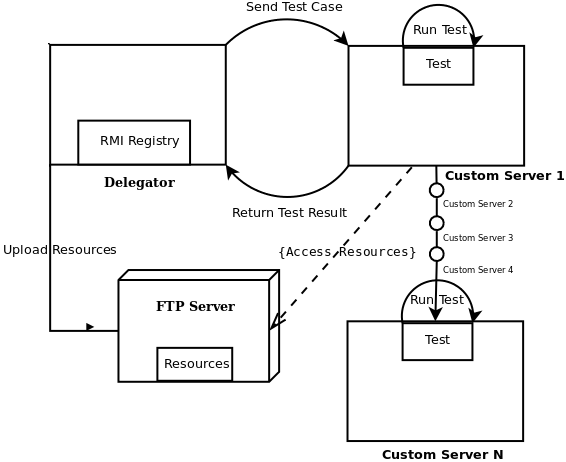
\includegraphics[width = \textwidth]{DTS_Diagram.png}
\caption{Architecture of the Distributed Test Sharer (DTS).}
\label{dtsdiagram}
\end{figure}

Before starting the system, the user is expected to furnish all of the JUnit test cases and any associated resources needed to run those test cases.  All files will be placed in the \texttt{ftpserver} directory, or one of its subdirectories.  The top level of this directory can be filled with any non-class files or directories that might be required for test suite execution.  For instance, the SchemaAnalyst test suite uses a \texttt{config} directory that contains various text files filled with different properties.  In this example, the user would place the entire \texttt{config} directory immediately inside the \texttt{ftpserver} directory.  Further nested in the \texttt{ftpserver} directory is a \texttt{resources} directory, which contains  \texttt{bin}, \texttt{lib}, \texttt{test\_singles} and \texttt{test\_suites} subdirectories.  For simplicity, the user should put the entirety of the directory containing their compiled classes in the \texttt{bin} directory.  Continuing with the SchemaAnalyst example, this would involve placing the \texttt{org}, \texttt{paper}, and \texttt{parsedcasestudy} directories into the \texttt{ftpserver/resources/bin} directory, which are usually located in that system's \texttt{build} directory.  All \texttt{jar} files used by the desired tests should be placed in the \texttt{lib} directory.  Finally, any individual JUnit test cases can be put in the \texttt{ftpserver/resources/test\_singles} directory, while any test suites (those that reference multiple JUnit test cases, like an \texttt{AllTests} class) can be put in the \texttt{ftpserver/resources/test\_suites} directory.

DTS execution begins on the side of the \texttt{Delegator} with a few preliminary steps.  First, several system properties are programmatically altered. These include \texttt{java.security.policy}, which is set to a custom policy that grants all permissions to any nodes that attempt to connect to the \texttt{Delegator} through Java RMI.  Although a more stringent policy would generally be recommended to improve the security of the system, this was deemed appropriate for the purpose of prototyping the system with fewer obstacles.  Further, the \texttt{java.rmi.server.hostname} property is set to the internet protocol (IP) address of the \texttt{Delegator}, which is retrieved through the command line interface at program execution.  This specifies the given IP address for use with any registry that is subsequently created, allowing remote nodes to find it.

Next, a Java RMI registry is created using a port number that is currently hard coded as 12345.  This port number was chosen because it resides in the range of acceptable ports for the machines used for experimentation, and generally is not assigned to any other system processes.  A new instance of \texttt{Delegator} is then created and linked to the registry through use of the \texttt{rebind()} method, binding the object with a key of "Delegator."  This will allow \texttt{CustomServer} nodes to access some of the methods offered by \texttt{Delegator} in future steps.

Both the \texttt{Delegator} and \texttt{CustomServer} classes extend \texttt{UnicastRemoteObject}, which allows them to be bound to and retrieved from a Java RMI registry.  It facilitates the dynamic creation of stubs for such objects, obviating the static method used in previous versions of Java.  Each class also implements an interface that extends \texttt{Remote}: \texttt{DelegatorInterface} and \texttt{CustomServerInterface}.  The \texttt{Remote} marker interface is further required to successfully bind to the registry, and it allows for type checking of remote object invocations at compile time.

After the registry is created, an FTP server is created using the Apache FtpServer framework.  This framework was chosen because it allows programmatic creation of an FTP server using Java, instead of relying on a third-party application that would need to be run and configured separately.  Various settings are adjusted during this step, such as establishing a user name and password, setting the port and host address, and enabling concurrent logins.  Most importantly, the home directory for the FTP server is set to the \texttt{ftpRootDir} variable, which is currently hard coded to the local \texttt{ftpserver} directory where the test cases and resources were previously placed.  Any users that connect successfully with the server will then have immediate access to this directory and any nested directories contained within it.

The final preliminary step taken by \texttt{Delegator} is the creation of a list of JUnit test cases.  Both the \texttt{ftpserver/resources/test\_singles} and \texttt{ftpserver/resources/test\_suites} are traversed recursively to locate all nested \texttt{class} files, which are saved as \texttt{File} objects and stored into separate global \texttt{LinkedLists}: \texttt{testSingleList} and \texttt{testSuiteList}.

After these steps are completed by the \texttt{Delegator}, it waits until the user enters the carriage return character to continue.  During this wait, remote nodes can connect to the \texttt{Delegator} by running the \texttt{CustomServer} class.  Importantly, two command line arguments must be specified at execution: the IP address of the \texttt{Delegator}, followed by the server's own IP address.  Ideally, multicasting would be used by the \texttt{Delegator} to broadcast its address, allowing the \texttt{CustomServers} to locate it automatically.  While this might be pursued in the future, the current implementation requires the \texttt{Delegator's} IP address to be known.  

Once started, the \texttt{CustomServer} sets the system RMI policy in the same manner as done by the \texttt{Delegator}.  Additionally, it will set the \texttt{java.system.class.loader} system property to a \texttt{CustomClassLoader}.  This class extends a \texttt{URLClassLoader} and allows access to some of the normally protected methods through use of reflection.  For now, it simply sets the classpath to the local \texttt{bin} and \texttt{lib} directories.  Next, the \texttt{CustomServer} will locate the registry on the \texttt{Delegator}, using the IP address previously specified, and obtain a remote reference to the bound \texttt{Delegator} object using the \texttt{Naming.lookup()} method.  Using this reference, it will call the \texttt{rebindServer()} method to bind the \texttt{CustomServer} to the registry.  This is repeated for each \texttt{CustomServer} node until they are all bound to the registry.

After all \texttt{CustomServers} are created and connected, then the user will enter the carriage return character on the \texttt{Delegator} node to continue execution.  The \texttt{Delegator} will first call the remote \texttt{updateClassLoader()} method for each of the \texttt{CustomServers}.  This will add all of the relevant \texttt{class} directories and \texttt{jar} files to the classpath of each \texttt{CustomServer}, accessible via FTP protocol and the FTP server previously created.  Additionally, all of the non-class files previously placed in the \texttt{ftpserver} directory on the \texttt{Delegator} node are actively retrieved through communication with the FTP server and stored locally on each server node.  Although efforts were made to obviate the need to store any files on the server, this was deemed a critical step to ensure that subsequent tests could be run successfully.

Next, the \texttt{Delegator} creates \texttt{TestAgent} objects for each \texttt{CustomServer}.  These agents extend the \texttt{Thread} class and implement \texttt{Runnable}, allowing multiple agents to run their respective methods concurrently on separate threads.  The \texttt{run()} method will simply do a remote call to the \texttt{runTest()} method for its assigned \texttt{CustomServer}, sending a test case and storing the \texttt{Result} generated by the server into the same \texttt{ConcurrentLinkedQueue}.  These agents are further placed into another \texttt{ConcurrentLinkedQueue} for subsequent access by the \texttt{Delegator}.

Once these agents are created, the \texttt{Delegator} will sequentially iterate first through the \texttt{testSingleList}, and then through the \texttt{testSuiteList}.  With the single test cases, each \texttt{File} in the list is assigned as-is to an agent in the queue, provided that agent is not currently active.  The \texttt{run()} method of the agent is then started, sending the test to the assigned \texttt{CustomServer}.  If the agent is active, then it is placed back into the queue and the next agent is checked, continuing in that manner.  This load sharing approach ensures that each \texttt{TestAgent}, and therefore each \texttt{CustomServer}, is always running a single test case at all times.  This process is similarly repeated while iterating through the test suites, with some additional steps.  The test suite \texttt{File} is first converted into a byte array, which is then converted into a \texttt{Class} object using a \texttt{SimpleClassLoader}.  This class loader simply overrides the \texttt{defineClass()} method of a generic \texttt{ClassLoader}, allowing this conversion to take place.  Next, the test suite is further converted into an array of \texttt{Class} objects by retrieving all test cases listed under the \texttt{SuiteClasses} annotation in the suite.  This array, containing all of the individual test cases in the suite, is iterated through in the same manner described previously, performing load sharing using the previously created agents.

On the \texttt{CustomServer}, there are two \texttt{runTest()} methods: one has a \texttt{File} parameter, while one has a \texttt{Class} parameter.  The method for \texttt{Class} objects simply executes the static \texttt{JUnitCore.runClasses()} method on that object, which returns a \texttt{Result} object.  This \texttt{Result} object contains all of the details about the successes and failures from running the test, and is returned to the caller.  The \texttt{runTest()} method for \texttt{File} objects first converts the \texttt{File} to bytes, and then to a \texttt{Class} object, finally using the same \texttt{JUnitCore.runClasses()} method to run the test.  This is performed by the \texttt{CustomServer} to lessen the computation required on the \texttt{Delegator} as much as possible.  In both cases, running the tests is only possible due to the previously implemented \texttt{CustomClassLoader}.  This allows the JVM to automatically retrieve any needed \texttt{class} or \texttt{jar} files via communication with the FTP server on the \texttt{Delegator} without any prompting from the user, and without needing to copy those files to the \texttt{CustomServer} node.

The \texttt{Delegator} continues to perform load sharing, assigning test cases to \texttt{TestAgents}.  The agents continue to store the \texttt{Result} objects returned from the \texttt{runTest()} method of each \texttt{CustomServer} into the same \texttt{ConcurrentLinkedQueue}.  Once all tests have been assigned, and all \texttt{Results} have been retrieved, then the each \texttt{Result} is parsed and the total number of successes and failures are displayed for the user.  Each failure is further elaborated to show why a test case might have failed.  This completes the process used by the Distributed Test Sharer, with all tests located on the \texttt{Delegator} having been executed by separate, remote nodes.

\section{Experimentation Protocol}
\label{experiments}

\subsection{Systems Specifications}
\label{specs}

\begin{itemize}
\item \textbf{Colton's 13-inch, Mid 2012 MacBook Pro}
\begin{itemize}
    \item OS / Version: OS X El Capitan version 10.11.4
    \item Processor: 2.9 GHz Intel Core i7
    \item Memory: 8 GB 1600 MHz DDR3
    \item Startup Disk: Samsung 850 Pro SSD
\end{itemize}

\item \textbf{Herbie's Hp Envy TS 17 Notebook PC}
\begin{itemize}
    \item OS / Version: 64-bit Windows 10
    \item Processor: 2.4 GHz Intel Core i7-4700MQ
    \item Memory: 16 GB
    \item Startup Disk: Samsung 850 Pro SSD
\end{itemize}

\item \textbf{Herbies's HP Dv7-6c95dx Notebook PC}
\begin{itemize}
    \item OS / Version: 64-bit Windows 10
    \item Processor: 2.20 GHz 2nd generation Intel Core i7-2670QM
    \item Memory: 8 GB
    \item Startup Disk: Samsung 280 Pro SSD
\end{itemize}

\item \textbf{Herbie's Fujitsu lifebook t2020 (x2)}
\begin{itemize}
    \item OS / Version: 32-bit Ubuntu 14.04
    \item Processor: 1.2 GHz Intel Core 2 Duo U9400
    \item Memory: 3 GB
\end{itemize}
\item \textbf{Michael's Dell Inspiron}
\begin{itemize}
    \item OS / Version: 64-bit Windows 8.1
    \item Processor: 2.16 GHz Intel Core Duo Celeron n2830
    \item Memory: 4 GB
\end{itemize}
\end{itemize}

\subsection{Experimentation Protocol for TLB}
For TLB we ran a Docker container with Java SE Development Kit 8u91 and Apache Ant version 1.9.4. These were both necessary
for running the existing tool in the Test Load Balancer (TLB). TLB is compatible with JDK versions as old as version 6, but
to keep our experiments as consistent as possible, we installed the latest version (8u91) on all of the machines being used for
testing. Having the newest version of Apache Ant was not entirely necessary, but again, we wanted to have the most
recent versions of software for this experiment due to possible optimizations in the newest versions.

\subsubsection{Running TLB in a Distributed Fashion}
We ran the TLB tool five times for all configurations (e.g. three nodes on the schema-analyst test suite). We decided
to only run each configuration five times due to time constraints. We had it calculated that if we ran each configuration
for the thiry trials suggested by Traeger et al. that our experiments combined would take approximately 20-hours
to run, requiring us to sit at our computers and monitor the tests constantly for this amount of time \cite{traeger2008nine}.

Also, for the TLB experimentation setup, we ran Docker containers on each node. There were three total nodes, all of which
were the available personal laptops of a team member. The system specifications for the machines used in this experiment
can be found in section \ref{specs}. We would have liked to run the experiments in a more controlled and consistent environment
by running the Docker containers with TLB on the Alden lab machines, but were denied permission to install Docker for various
potential security reasons. To read more about the challenges faced during this assignment, read section \ref{challenges}.

The way TLB is designed requires a user to start the \texttt{TLBServer} on one node and start the clients with the \texttt{TLBBalancer}
on other nodes. Therefore, to collect the data necessary, we started the server on the 13-inch, Mid 2012 MacBook Pro
and ran the Docker containers on two other machines as well as on the MacBook Pro. This was the setup for running three
clients with the TLB system. For two and a single client, we removed Michael's Dell Inspiron,  which performed the
worst when running the test suites in the Docker container. Specifically, for two nodes, we used Herbie's HP Envy
as one client node and Colton's MacBook Pro as the other client as well as the server.
Ideally, we would have liked to only run the server on Colton's MacBook Pro and the clients on their own
individual machines, but again, Michael's laptop took substantially longer time to execute its portion of the test suite.
However, for a single node, we did not have to worry about running a server on a different machine. We ran the Apache Ant
task \texttt{test} which for SchemaAnalyst's test suite called five iterations of the test suite and for Apache Ivy
ran the test suite provided with the system.

It was the case that in order to make test suite execution time long enough to see substantial differences between
number of nodes, we needed to run multiple iterations of the same test to artificially increase test suite execution
time. Additionally, for comparison to a test-sharing system we needed to run this modified version of SchemaAnalyst's
test suite.

This is the protocol we followed throughout the experimentation phase of this final laboratory assignment. We acknowledge that
there were a lot of places where we did not apply the industry-standard protocols for testing, however due to time constraints
and availability of machines, this is the best protocol that we could follow to ensure that the data that we collect
was as accurate and consistent as possible.

\subsection{Experimentation Protocol for DTS}
Similar to running TLB, there were many steps that were taken to ensure that the quality of experimentation for DTS was the highest possible. While running tests for a distributed test suite it is important to consider the fact that outside factors may have an impact on the results. Since this is the case, we listed all possible factors which could hinder a smooth analysis of the program. We then used our knowledge of these potential problems to minimize their impact. 
\subsubsection{Running DTS in a Distributed Fashion}
The first step in our experimentation was choosing nodes which could host our system. The computer system implemented in Alden Hall at Allegheny College was unable to run our customized system. Since this was the case we chose to gather personal computers from different group members for testing. The difference in testing between our DTS and TLB is that some computers which were viable for DTS were not viable for TLB. The computers used for DTS testing were Herbie's HP Envy, Herbie's DV7, Herbie's Fujitsu Lifebook X2, and Michael's Dell Inspiron. Since the format of our implementation has a delegator, we set aside Herbie's HP Envy solely for this purpose. This means that we had a total of 4 nodes to start running the tests on.

 As mentioned previously, these computers ran different operating systems. This means it was necessary to configure the operating systems separately. The main concern was that automatic updates and background processes were double checked to be inactive during testing. After this was done, we were able to run the tests for 5 trial per number of nodes. To clarify, we ran 5 good trials for each 4,3,2,and 1 node. While doing this it is important to note that the network used for this experiment was public. Since the network was public we had to ensure that the network was not being slowed by other users. In order to combat this situation we ran the tests on the network around 5 A.M Eastern Time on a Saturday. This would most likely be the least active time for the network on a college campus. Each test from this point was run successfully while considering a few different things.
 
 The first thing to consider was that data may be cached after running the program multiple times. In order to combat this we ran the program 5 times before collecting any data. Another concern was that Java's garbage collector would interfere. This being said, we discarded any data was more than 8 percent deviation from the average since it is very difficult to infer what data is being skewed by the garbage collector. The tests run on 4 nodes was run with all computers. The tests run on 3 nodes was run with Herbie's DV7 and T2020 X2 laptops. The tests run on 2 nodes was run with the T2020 lifebooks only. This was reduced to a single T2020 lifebook for the single node.
 
 Similar to testing the TLB system, there were places where we did not follow industry standards of testing. We acknowledge that there may be some cases that need further explored. However,as talked about above, we did try to combat this at every possible instance. Overall, experimentation with the DTS system was a success and the results of these experiments are further analysed in the next section,
\section{Analysis of Results}
\label{analysis}

The first analysis will be of running Apache Ivy's test suite on the Test Load Balancer tool.
On average, on one node, running the Apache Ivy test suite took approximately six minutes to
execute. To clarify, when I refer to running on a single node, I am referring to running the
test suite using the \texttt{ant test} task in the \texttt{build.xml} instead of the \texttt{ant test.load.balanced}
task.

Where we expected to see a significant performance increase---especially with the Apache Ivy test suite---
was when adding additional nodes. However, we did not see this dramatic increase in performance
and actually experienced a decrease in performance when adding the third node. I will note
that the third node that was added was Michael's Dv7-6c95dx which we noticed took substantially
longer to execute test suites than other nodes on average.

Therefore, we see the greatest performance when balancing the work using the Test Load Balancer tool
to two nodes. When executing the Apache Ivy test suite on two remote nodes, we notice that each
node is able to complete their portion of the test in approximately 1.25 minutes. Refer to Figures
\ref{ivybar} and \ref{ivybox}.


\begin{figure}[!ht]
  \centering
  \begin{minipage}[b]{0.4\textwidth}
    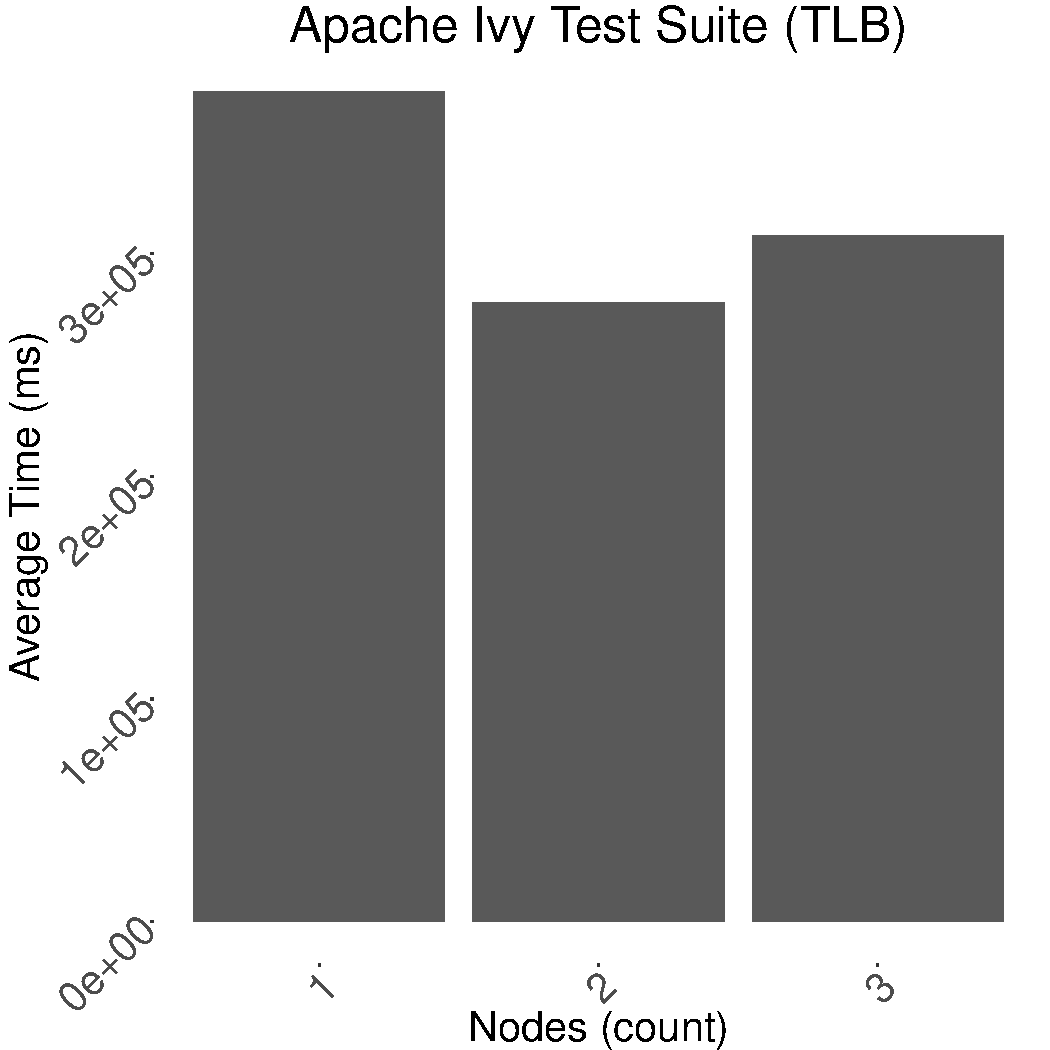
\includegraphics[width=\textwidth]{../data/graphs/ivy_bar_tlb.pdf}
    \caption{A bar chart displaying average time in milliseconds to run Apache Ivy's test suite on TLB}
    \label{ivybar}
  \end{minipage}
  \hfill
  \begin{minipage}[b]{0.4\textwidth}
    \includegraphics[width=\textwidth]{../data/graphs/ivy_boxplot_tlb.pdf}
    \caption{A boxplot displaying average time in milliseconds to run Apache Ivy's test suite on TLB}
    \label{ivybox}
  \end{minipage}
\end{figure}

Secondly, and more importantly, we wanted to analyze the effectiveness of the Test Load Balancer tool
at balancing SchemaAnalyst's test suite. This is more important to use in particular because
the Distributed Test Sharing tool is---in its current state---only able to execute this test suite.
With that said, we are able to compare direct performances of the tools. However, again, there are
some inconsistencies such as which laptops were available for the systems to be run on.

Similarly to the Apache Ivy's test suite for the Test Load Balancing tool, the TLB tool experiences
its best performance with two nodes. We hypothesize that this is for the same reason as noted previously
regarding to the performance of the one node. However, here when the third node is introduced, running the
test suite locally, one a single node is more performant. This makes it not worth distributing tests to
more than two nodes.

SchemaAnalyst's test suite on a single node took on average 15 seconds to execute. We do note that there
are a lot of failing tests and missing resources. This is why we hypothesize that this execution time
is so minimal. A lot of the dependencies necessary for this test suite are database management systems
that were not installed on many of the machines used in this experiment.

In conlusion, for the TLB tool, it is not worth running either Apache Ivy's or SchemaAnalyst's test suite
on more than two nodes. For both of these test suites, it is worth balancing the work to two
remote nodes using the TLB tool communicating with the TLBServer to \texttt{POST, PUT} and \texttt{GET} historical
test data for a given test suite.

\begin{figure}[!ht]
  \centering
  \begin{minipage}[b]{0.4\textwidth}
    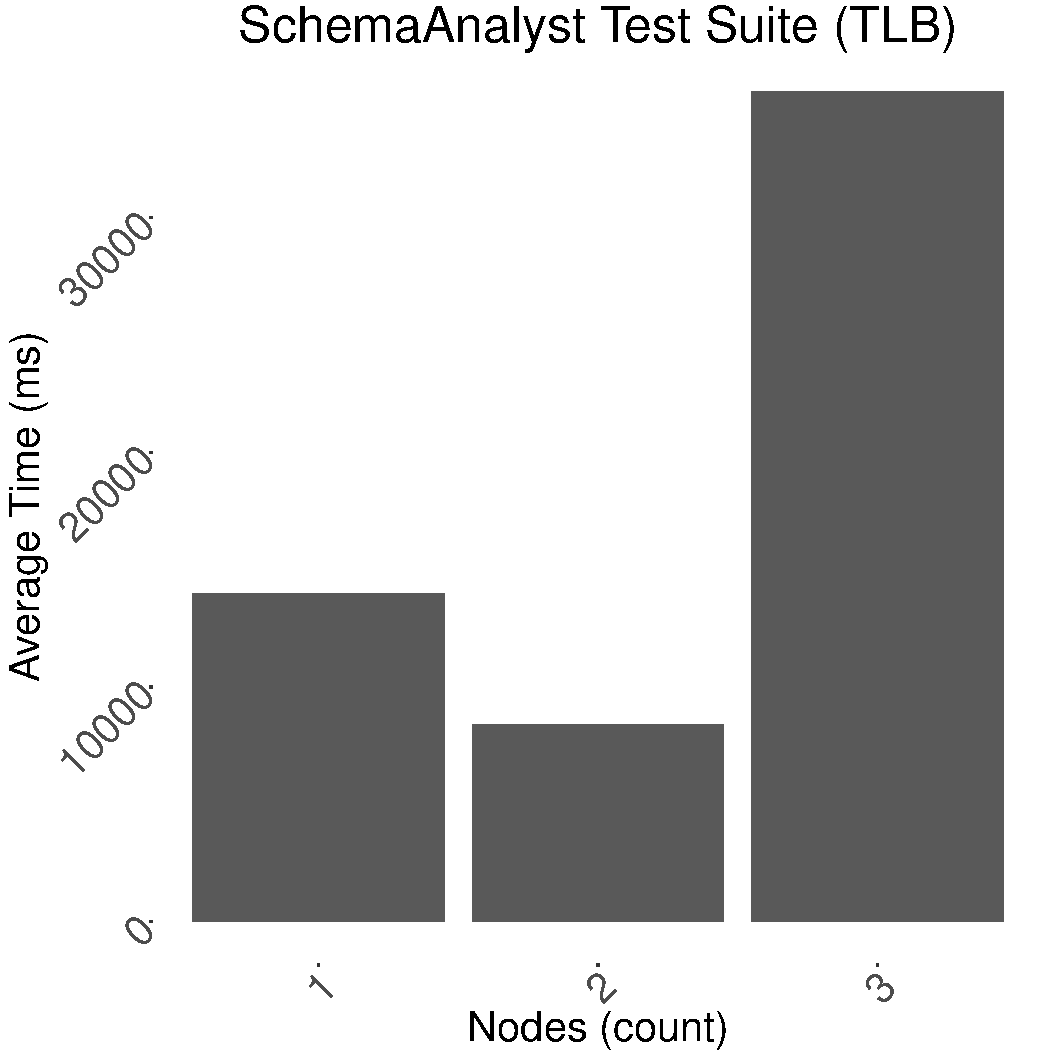
\includegraphics[width=\textwidth]{../data/graphs/sa_bar_tlb.pdf}
    \caption{A bar chart displaying average time in milliseconds to run SchemaAnalyst's test suite on TLB}
    \label{sabar}
  \end{minipage}
  \hfill
  \begin{minipage}[b]{0.4\textwidth}
    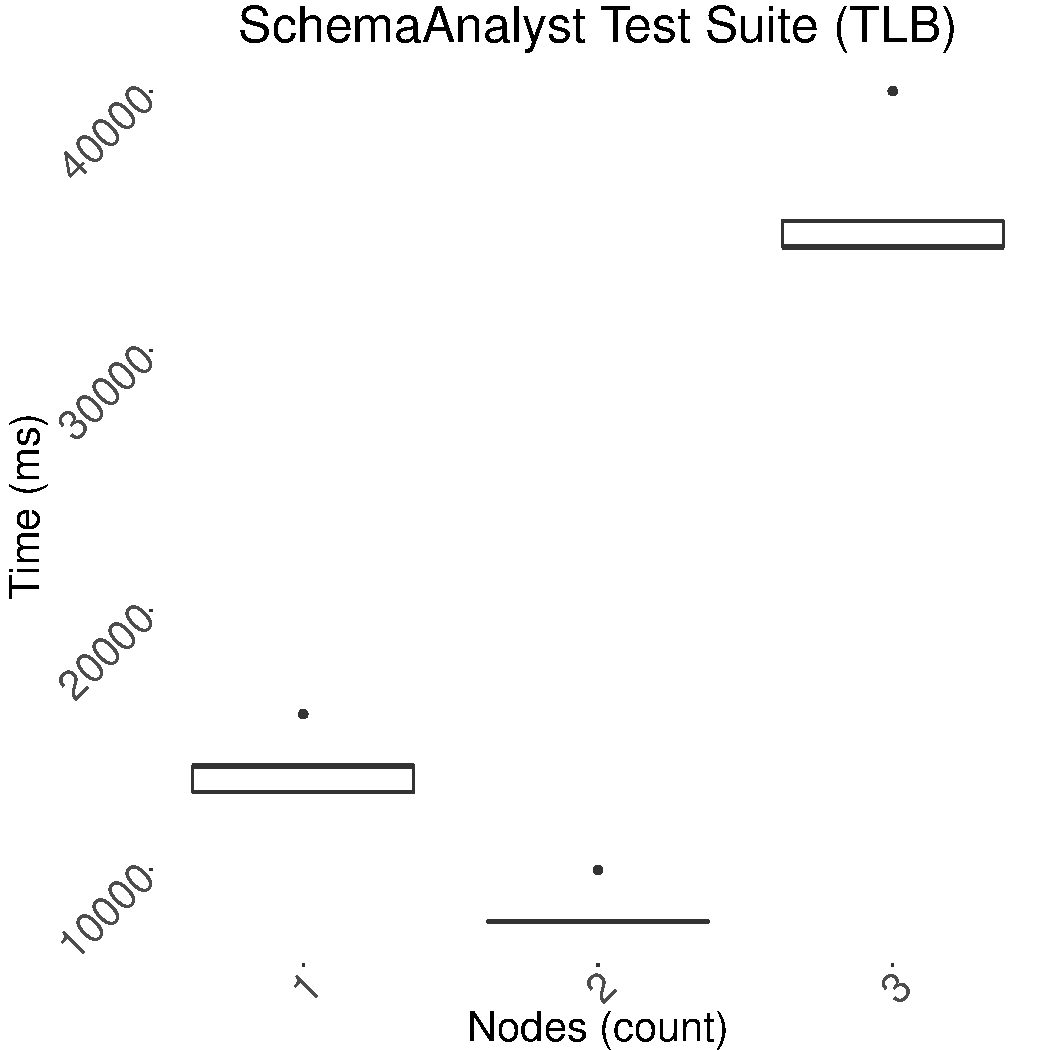
\includegraphics[width=\textwidth]{../data/graphs/sa_boxplot_tlb.pdf}
    \caption{A boxplot displaying average time in milliseconds to run SchemaAnalyst's test suite on TLB}
    \label{sabox}
  \end{minipage}
\end{figure}

\begin{figure}[!ht]
  \centering
  \begin{minipage}[b]{0.4\textwidth}
    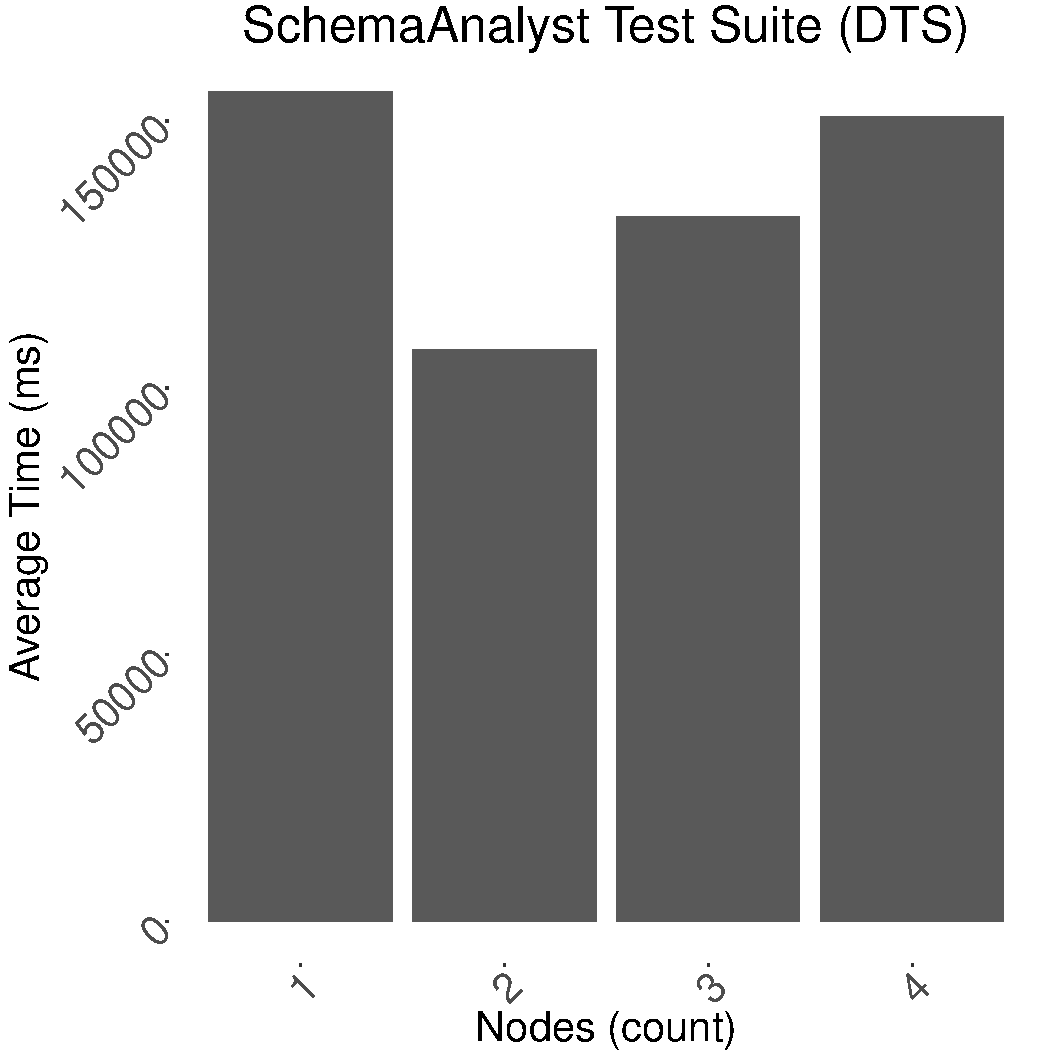
\includegraphics[width=\textwidth]{../data/graphs/sa_bar_dts.pdf}
    \caption{A bar chart displaying average time in milliseconds to run SchemaAnalyst's test suite on DTS}
    \label{sabardts}
  \end{minipage}
  \hfill
  \begin{minipage}[b]{0.4\textwidth}
    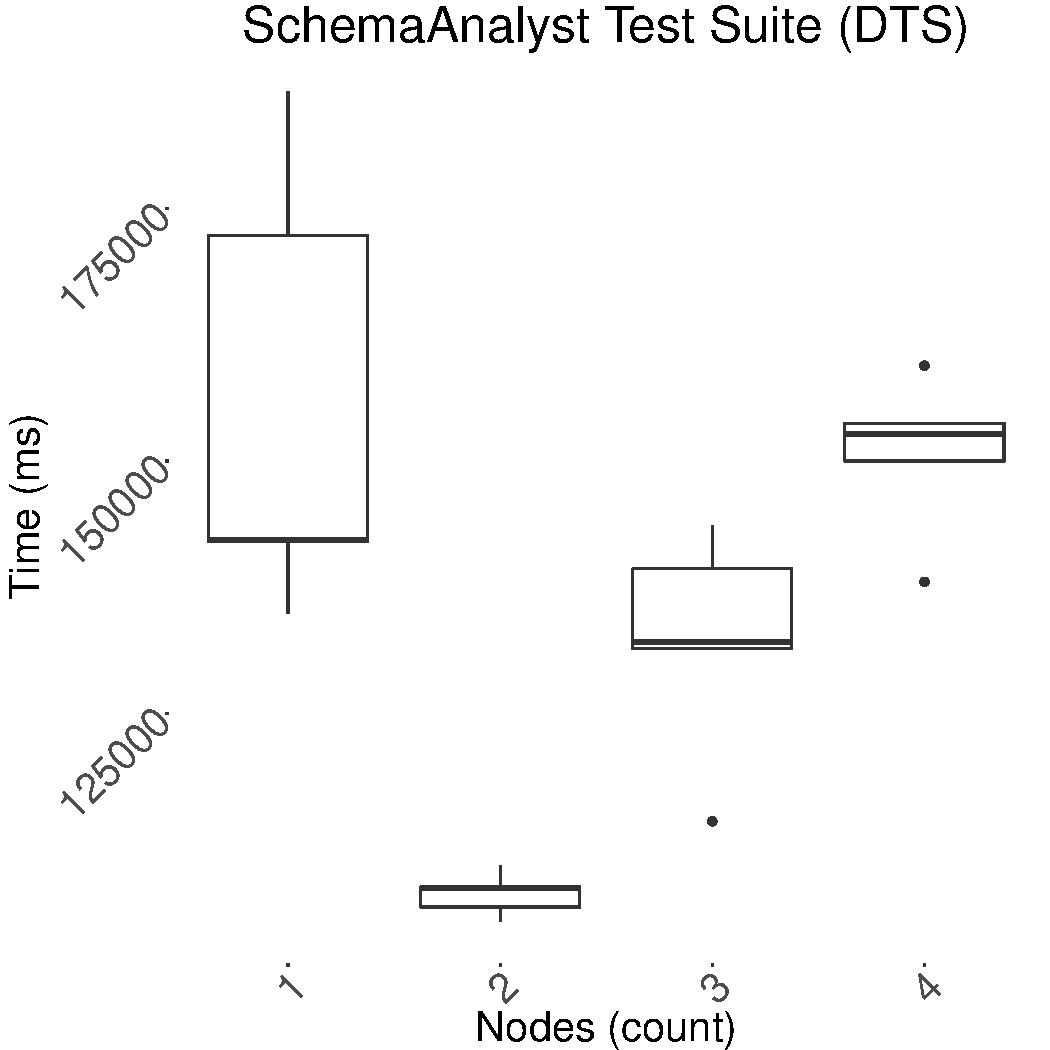
\includegraphics[width=\textwidth]{../data/graphs/sa_boxplot_dts.pdf}
    \caption{A boxplot displaying average time in milliseconds to run SchemaAnalyst's test suite on DTS}
    \label{saboxdts}
  \end{minipage}
\end{figure}

Finally, we are interested in the performance of the system created by Michael, Distributed Test Sharer (DTS).
As previously noted, we were only able to run SchemaAnalyst's test suite on DTS.

First, in Figures \ref{sabardts} and \ref{saboxdts}, we see that running the test suite on a single node takes
about 2.5 minutes to execute. Then, we notice that when sharing the work with another node, we see a pretty
substantial performance increase, reducing the overall time to execute the test suite to a little
over a minute and a half. This is a total reduction of about a whole minute.

However, we see a trend when observing these visualizations. We notice that as we add more nodes to share work
with there is a direct correlation to the increase in time to execute the test suite. This is due
to the overwhelming communication costs between these larger number of nodes. We are able to eliminate
the costs of actually transferring the files necessary for running the test suite by accessing them through
a file transfer protocol. Had we added this additional cost on top of already expensive communication, running
the DTS tools as a sharing mechanism for SchemaAnalyst's test suite would make it less worth much more quickly.

\begin{figure}[!ht]
    \centering
    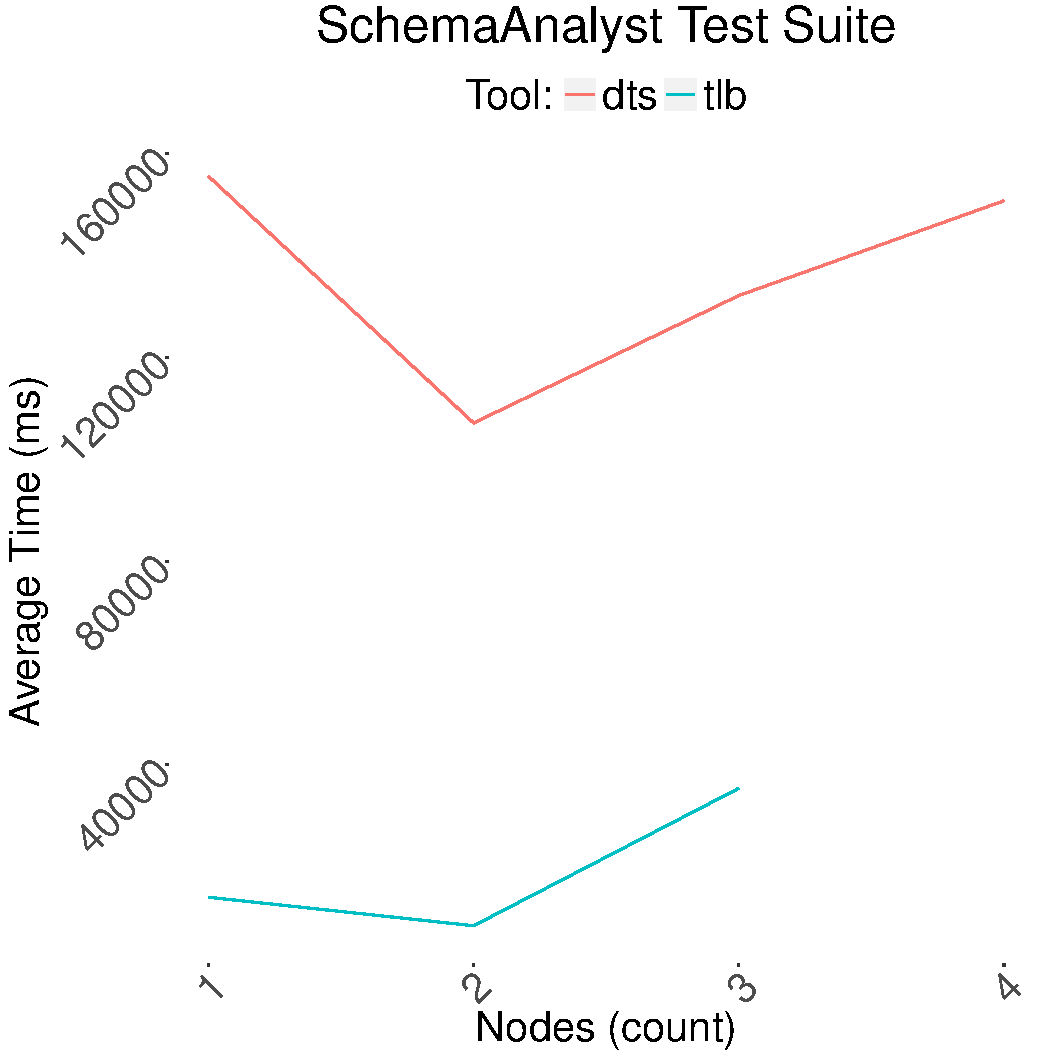
\includegraphics[scale = 0.5]{../data/graphs/line_both.pdf}
    \caption{A direct performance comparison of the TLB and DTS tools for running SchemaAnalyst's test suite}
    \label{lineboth}
\end{figure}

In Figure \ref{lineboth}, we notice that both TLB and DTS behave similarly when distributing the SchemaAnalyst test
suite. Running the test suite on a single node takes longer than the most performant number of nodes---that being
two total nodes. At two nodes, both systems perform their absolute best and only decrease in overall performance
from there.

Remember, we were limited to only comparing the test suite of the SchemaAnalyst tool and on very few nodes due to
the lack of permissions and available resources. We would have liked to run these two systems on many more
similar nodes to alleviate any inconsistencies, however this was just not possible for the scope of
this final laboratory assignment.

\section{Challenges}
\label{challenges}

Various challenges were encountered while developing the Distributed Test Sharer, with many of these challenges revolving around the use of Java RMI for communication between nodes.  There were a variety of different settings and properties that I didn't originally know about, despite using this technique in a previous assignment.  These included either setting the RMI host name and security policy through the \texttt{-Djava} command line parameter, or using the \texttt{System.setProperty()} method programmatically.  Omitting these steps produced a variety of different, confusing errors, and required much troubleshooting to figure out how to fix them.  There were also problems getting the RMI to work on the computers in Alden Hall, which ultimately prevented those computers from being used in our experiments.  Originally, these problems arose from the fact that the Java RMI registry would occasionally use a random port number instead of the one specified in the source code.  This created much confusion originally, since the Java API includes various method signatures that require a port number parameter; yet it seemed as though such specification did not have the expected effect.  Ultimately, using a custom \texttt{SocketServerFactory} and adjusting the parameters for the \texttt{UnicastRemoteObject} constructor fixed those initial problems involving randomly assigned ports.  However, new problems arose with remote objects being removed from the registry after binding, perhaps due to some garbage collection issue.  These problems were not present during testing of DTS on personally owned computers, and unfortunately they could not be resolved despite significant time investment.

Another challenge with DTS was getting the tests to run on a separate node without error, and specifically without needing to copy over any files to the servers.  I used a custom \texttt{URLClassLoader} to originally overcome this challenge, which is a vital component to the system.  Although this allows the JVM to access the FTP server for \texttt{class} and \texttt{jar} file, it doesn't redirect the paths used for other kinds of files.  For instance, the SchemaAnalyst test suite makes use of a \texttt{config} directory that contains various properties files.  Although I could specify the exact FTP URL for the class loader to locate this directory, the test cases would not find it when they ran on the server.  I tried to adjust the system property for the current working directory (\texttt{user.dir}), among other fixes, but could never bypass this error completely.  Ultimately, in order to get the tests to work as expected, I need to add a step to the \texttt{updateClassLoader()} method on the \texttt{CustomServers} to retrieve and store some files from the FTP server.  This was unfortunate, since a notable benefit of this system is the lack of resource overhead for the servers; but it was necessary in order to have a functional system within our time constraints.  This general issue with file dependencies further complicated running DTS on complex systems like \texttt{ant-ivy} and \texttt{tomcat}, despite the accommodations made to DTS.  The prevented DTS to be run on similar systems as TLB, and it would be one of the first areas of improvement if development on this system were to continue.

In addition to the challenges Michael encountered while implementing the DTS tool, there were similar challenges
faced while configuring, analyzing and running the existing, Test Load Balancing tool.

First, while the system is on GitHub (\url{https://github.com/test-load-balancer/tlb}), it is not a working version. GitHub is initially where I found the tool, but in the
tool repository the creators direct you to the tool website (\url{http://test-load-balancer.github.io/}). The tool website is
filled with data and comments about the tool, however when it came time to configuring and running the tool, these
processes were not made absolutely clear. No where on this page does it say they do not support actually running the
clients in a distributed fashion.

Also, while there is a configuration page containing documentation for all of the necessary environment variables,
the provided examples and descriptions are not clear at describing all of the variables. Luckily, we were
able to reach out and hear back from the creators of this tool. They were able to guide us in the correct
direction. But even without the help of the authors, we were able to find the answer to our question
regarding how to configure the distribution of a test suite using the TLB tool was answered in a blog
post by one of the creators of the TLB tool. Even here though, there were only one or two sentences
on the topic. Maybe it was made clear somewhere else, but to me, this fact was not evident.

In order to run the TLB tool in a distributed fashion, we were required to use multiple nodes.
We were able to accomplish this by creating containers---which are virtually easy-to-configure
virtual machines with all of the necessary dependencies for running TLB. While we did run
into one issue with Docker, that being installing Docker on a 32-bit machines, overall,
Docker was a pretty easy-to-use system, especially for Mac OS X.

As mentioned, the only issue we had with Docker directly was when trying to install it on an unsupported
build of Windows. To combat this compatibility issue, we asked permission to have Docker
installed on the Alden lab machines. If Docker were installed on the lab machines,
our experiments would have been much more interesting, consistent and more detailed.

The final issue that I encountered was when trying to run experiments. I knew the TLB tool had
been working the evening before trying to run the experiments and I had not manipulated any of
the files and the TLB system was not communicating or running the test suites. I tried a number of
ports to no avail. Finally, I decided to try the system at home once again and everything worked
flawlessly, therefore requiring me to haul all of the necessary machines for the experiment
to my house.

\section{Conclusion}
\label{conclusion}

\section{Appendix}
\label{appendix}

\subsection{Data}
\newpage
\verbatiminput{../data/tlb-data.csv}
\newpage
\verbatiminput{../data/dts-data.csv}

\newpage
\subsection{Representative Source Code}
\verbatiminput{../container/Dockerfile}
\newpage
\inputminted{xml}{../container/tlb/tools/schemaanalyst/build.xml}
\newpage
\inputminted{bash}{../container/tlb/tools/schemaanalyst/run_balanced.sh}
\inputminted{bash}{../container/tlb/tools/recipe.sh}
\newpage
\inputminted{xml}{../container/tlb/tools/ivy/build.xml}

% \inputminted{java}{../simple-rmi/src/Simple.java}

% Generate the bibliography.
\bibliography{bibliography}
\bibliographystyle{unsrt}

\end{document}
